\chapter{Analysis and Specification of Requirements}
\setcounter{minitocdepth}{1}
\minitoc
\newpage

\section{Introduction}
This section aims to define and categorize the essential requirements of the project, distinguishing between functional requirements, which describe specific behaviors and capabilities of the system, and non-functional requirements, which focus on performance, security, accessibility criteria, and other overall qualities.

\section{Functional Requirements}
\section{Functional Requirements}
The functional requirements of our solution include the features that it must incorporate to meet the project's requirements and objectives. These requirements are essential for ensuring that the system performs the necessary tasks effectively.

The system must offer \textbf{shop visitors} the possibility to:

\begin{itemize}
    \item View Shop
    \begin{itemize}
        \item View the shop's products.
        \item View the shop's categories.
        \item Search for products.
        \item View the product's details.
        \item Add products to the cart.
        \item View the cart.
        \item Accept or decline upsells.
    \end{itemize}
\end{itemize}

The system must offer \textbf{shop owners} the possibility to:

\begin{itemize}
    \item Manage upsells
    \begin{itemize}
        \item Add upsells.
        \item Edit upsells.
        \item Delete upsells.
        \item View upsells preview.
        \item Search for upsells.
    \end{itemize}
    
    \item Manage Orders
    \begin{itemize}
        \item View orders.
        \item Search for orders.
        \item View order details.
        \item Change order status.
        \item Filter orders.
    \end{itemize}
    
    \item Manage Budgets
    \begin{itemize}
        \item View budget list.
        \item Select budget.
        \item Edit budget information.
        \item View total balance, expenses, and incomes.
    \end{itemize}
    
    \item Manage Costs
    \begin{itemize}
        \item Input various costs.
        \item Calculate total costs.
    \end{itemize}
    
    \item Manage Notifications
    \begin{itemize}
        \item View notifications.
        \item Edit notifications sound.
    \end{itemize}
    
    \item View Statistics
    \begin{itemize}
        \item View statistics.
        \item Filter statistics.
    \end{itemize}
\end{itemize}

Having outlined the functional requirements, it is also crucial to consider the non-functional requirements that ensure the system's overall performance and quality.

\section{Non-functional Requirements}
The non-functional requirements of the system are as follows:
\begin{itemize}
    \item Performance: The system should be able to handle a large number of users and transactions without significant delays.
    \item Security: The system should protect sensitive data, such as customer information and financial records, from unauthorized access or theft.
    \item Scalability: The system should be able to grow and adapt to changing business needs, such as increased traffic or new features.
    \item Reliability: The system should be available and operational at all times, with minimal downtime or disruptions.
    \item Usability: The system should be easy to use and navigate, with clear instructions and intuitive interfaces.
\end{itemize}

\section{Analysis of Requirements}
This section provides an in-depth analysis of the system's requirements, identifying the key actors and their interactions with the system.

\subsection{Identification of System Actors}
The system involves the following actors, as detailed in Table \ref{tab:actors}:

\begin{table}[H] % Force table to appear where it is in the text
\centering
\begin{tabular}{|p{0.3\linewidth}|p{0.65\linewidth}|} % Adjusted column widths
\hline
\textbf{Actor} & \textbf{Description} \\
\hline
Shop Owner & The owner of the shop who can customize the template, manage orders, manage upsells, view statistics, customize notifications, manage budget and costs. \\
\hline
Shop Visitor & A visitor who visits the shop built on top of the template. \\
\hline
Superadmin & A special user who takes over temporarily to solve issues related to upsells. \\
\hline
\end{tabular}
\caption{System Actors}
\label{tab:actors}
\end{table}

\subsection{Global Use Case Diagram}
The global use case diagram represents the interactions between the system and its actors, as shown in Figure \ref{fig:use_case_diagram}.
\begin{figure}[H]
  \centering
  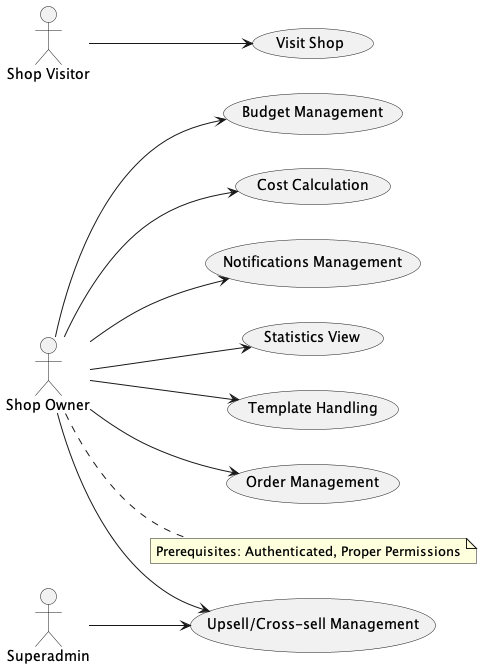
\includegraphics[width=0.5\textwidth]{Images/globalUseCase.png}
  \caption{Global Use Case Diagram}
  \label{fig:use_case_diagram}
\end{figure}

\subsection{Refinement of Use Cases}
It will be necessary to refine the already developed use case diagram to obtain more details about the features offered by the system and the constraints associated with them. This will allow us to better understand the system's behavior and interactions with its actors.

\subsubsection{Use Case 1: View Shop}
\begin{longtable}{|p{0.2\linewidth}|p{0.75\linewidth}|}
\hline
\textbf{Title} & Visit Shop \\
\hline
\textbf{Summary} & This use case describes the actions performed by a shop visitor to view the shop's products and categories, search for products, view product details, add products to the cart, view the cart, and accept or decline upsells. \\
\hline
\textbf{Actors} & Shop Visitor \\
\hline
\textbf{Preconditions} & The shop visitor has accessed the shop's website. \\
\hline
\textbf{Postconditions} & The shop visitor has viewed the desired products, added products to the cart, and accepted or declined upsells. \\
\hline
\textbf{Nominal Scenario} & 
\begin{enumerate}
    \item The shop visitor opens the shop's website.
    \item The shop visitor views the shop's products.
    \item The shop visitor views the shop's categories.
    \item The shop visitor searches for products.
    \item The shop visitor selects a product to view its details.
    \item The shop visitor adds the product to the cart.
    \item The shop visitor views the cart.
    \item The shop visitor accepts or declines upsells.
\end{enumerate} \\
\hline
\textbf{Alternative Scenarios} & 
\begin{itemize}
    \item The shop visitor does not find the desired products or categories.
    \item The shop visitor does not find any search results.
    \item The shop visitor encounters an error while adding a product to the cart.
    \item The shop visitor encounters an error while viewing the cart.
\end{itemize} \\
\hline
\end{longtable}

\subsubsection{Use Case 2: Manage Upsells}
\begin{longtable}{|p{0.2\linewidth}|p{0.75\linewidth}|}
\hline
\textbf{Title} & Manage Upsells \\
\hline
\textbf{Summary} & This use case describes the actions performed by a shop owner to add, edit, delete, view, and search for upsells. \\
\hline
\textbf{Actors} & Shop Owner \\
\hline
\textbf{Preconditions} & 
\begin{itemize}
    \item The shop owner has logged into the system.
    \item The shop owner has accessed the upsells management section.
    \item The shop owner has the appropriate permissions to manage upsells.
\end{itemize} \\
\hline
\textbf{Postconditions} & The shop owner has managed the upsells according to the desired actions. \\
\hline
\textbf{Nominal Scenario} &
\begin{enumerate}
    \item The shop owner logs into the system.
    \item The shop owner adds an upsell.
    \item The shop owner edits an upsell.
    \item The shop owner deletes an upsell.
    \item The shop owner views the upsells preview.
    \item The shop owner searches for upsells.
    \item The shop owner logs out of the system.
\end{enumerate} \\
\hline
\textbf{Alternative Scenarios} &
\begin{itemize}
    \item The shop owner encounters an error while adding an upsell.
    \item The shop owner encounters an error while editing an upsell.
    \item The shop owner encounters an error while deleting an upsell.
    \item The shop owner does not find any search results.
\end{itemize} \\
\hline
\end{longtable}

\subsubsection{Use Case 3: Manage Orders}
\begin{longtable}{|p{0.2\linewidth}|p{0.75\linewidth}|}
\hline
\textbf{Title} & Manage Orders \\
\hline
\textbf{Summary} & This use case describes the actions performed by a shop owner to view orders, search for orders, view order details, change order status, and filter orders. \\
\hline
\textbf{Actors} & Shop Owner \\
\hline
\textbf{Preconditions} & 
\begin{itemize}
    \item The shop owner has logged into the application.
    \item The shop owner has accessed the orders management tab.
    \item The shop owner has the appropriate permissions to manage orders.
\end{itemize} \\
\hline
\textbf{Postconditions} & The shop owner has managed the orders according to the desired actions. \\
\hline
\textbf{Nominal Scenario} &
\begin{enumerate}
    \item The shop owner logs into the system.
    \item The shop owner views the orders.
    \item The shop owner searches for orders.
    \item The shop owner selects an order to view its details.
    \item The shop owner changes the order status.
    \item The shop owner filters the orders.
    \item The shop owner logs out of the system.
\end{enumerate} \\
\hline
\textbf{Alternative Scenarios} &
\begin{itemize}
    \item The shop owner does not find any orders.
    \item The shop owner does not find any search results.
    \item The shop owner encounters an error while viewing order details.
    \item The shop owner encounters an error while changing the order status.
\end{itemize} \\
\hline
\end{longtable}

\subsubsection{Use Case 4: Manage Budgets}
\begin{longtable}{|p{0.2\linewidth}|p{0.75\linewidth}|}
\hline
\textbf{Title} & Manage Budgets \\
\hline
\textbf{Summary} & This use case describes the actions performed by a shop owner to view the budget list, select a budget, edit budget information, and view the total balance, expenses, and incomes. \\
\hline
\textbf{Actors} & Shop Owner \\
\hline
\textbf{Preconditions} & 
\begin{itemize}
    \item The shop owner has logged into the application.
    \item The shop owner has accessed the budgets management section.
    \item The shop owner has the appropriate permissions to manage budgets.
\end{itemize} \\
\hline
\textbf{Postconditions} & The shop owner has managed the budgets according to the desired actions. \\
\hline
\textbf{Nominal Scenario} &
\begin{enumerate}
    \item The shop owner logs into the system.
    \item The shop owner views the budget list.
    \item The shop owner selects a budget.
    \item The shop owner edits the budget information.
    \item The shop owner views the total balance, expenses, and incomes.
    \item The shop owner logs out of the system.
\end{enumerate} \\
\hline
\textbf{Alternative Scenarios} &
\begin{itemize}
    \item The shop owner does not find any budgets.
    \item The shop owner encounters an error while selecting a budget.
    \item The shop owner encounters an error while editing the budget information.
\end{itemize} \\
\hline
\end{longtable}

\subsubsection{Use Case 5: Manage Costs}
\begin{longtable}{|p{0.2\linewidth}|p{0.75\linewidth}|}
\hline
\textbf{Title} & Manage Costs \\
\hline
\textbf{Summary} & This use case describes the actions performed by a shop owner to input various costs and calculate the total costs. \\
\hline
\textbf{Actors} & Shop Owner \\
\hline
\textbf{Preconditions} & 
\begin{itemize}
    \item The shop owner has logged into the application.
    \item The shop owner has accessed the costs management section.
    \item The shop owner has the appropriate permissions to manage costs.
\end{itemize} \\
\hline
\textbf{Postconditions} & The shop owner has inputted various costs and calculated the total costs. \\
\hline
\textbf{Nominal Scenario} &
\begin{enumerate}
    \item The shop owner logs into the system.
    \item The shop owner inputs various costs.
    \item The shop owner calculates the total costs.
    \item The shop owner logs out of the system.
\end{enumerate} \\
\hline
\textbf{Alternative Scenarios} &
\begin{itemize}
    \item The shop owner encounters an error while inputting costs.
    \item The shop owner encounters an error while calculating the total costs.
\end{itemize} \\
\hline
\end{longtable}

\subsubsection{Use Case 6: Generate Financial Reports}
\begin{longtable}{|p{0.2\linewidth}|p{0.75\linewidth}|}
\hline
\textbf{Title} & Generate Financial Reports \\
\hline
\textbf{Summary} & This use case describes the actions performed by a shop owner to generate financial reports based on the inputted costs and revenues. \\
\hline
\textbf{Actors} & Shop Owner \\
\hline
\textbf{Preconditions} & 
\begin{itemize}
    \item The shop owner has logged into the application.
    \item The shop owner has inputted all relevant costs and revenues.
    \item The shop owner has accessed the financial reports section.
\end{itemize} \\
\hline
\textbf{Postconditions} & The shop owner has generated and reviewed the financial reports. \\
\hline
\textbf{Nominal Scenario} &
\begin{enumerate}
    \item The shop owner logs into the system.
    \item The shop owner navigates to the financial reports section.
    \item The shop owner selects the type of report to generate.
    \item The shop owner generates the financial report.
    \item The shop owner reviews the financial report.
    \item The shop owner logs out of the system.
\end{enumerate} \\
\hline
\textbf{Alternative Scenarios} &
\begin{itemize}
    \item The shop owner encounters an error while generating the financial report.
    \item The shop owner finds discrepancies in the financial report and needs to re-input data.
\end{itemize} \\
\hline
\end{longtable}

\subsubsection{Use Case 7: View Statistics}
\begin{longtable}{|p{0.2\linewidth}|p{0.75\linewidth}|}
\hline
\textbf{Title} & View Statistics \\
\hline
\textbf{Summary} & This use case describes the actions performed by a shop owner to view statistics and filter statistics. \\
\hline
\textbf{Actors} & Shop Owner \\
\hline
\textbf{Preconditions} &
\begin{itemize}
    \item The shop owner has logged into the application.
    \item The shop owner has accessed the statistics section.
\end{itemize} \\
\hline
\textbf{Postconditions} & The shop owner has viewed statistics and filtered statistics. \\
\hline
\textbf{Nominal Scenario} &
\begin{enumerate}
    \item The shop owner logs into the system.
    \item The shop owner views statistics.
    \item The shop owner filters statistics.
    \item The shop owner logs out of the system.
\end{enumerate} \\
\hline
\textbf{Alternative Scenarios} &
\begin{itemize}
    \item The shop owner does not find any statistics.
    \item The shop owner encounters an error while filtering statistics.
\end{itemize} \\
\hline
\end{longtable}

\section{Conclusion}
This chapter has provided an analysis and specification of the requirements for the project. It has identified the functional and non-functional requirements of the system, as well as the actors involved in the system. The global use case diagram has been presented, along with the refinement of use cases to provide more detailed information about the system's features and constraints. By thoroughly understanding these requirements and use cases, we can ensure that the system will meet the needs of its users and provide a robust, efficient, and user-friendly solution.